%% UniMind -- IEEE Transactions on Computers submission draft (full v2)
%% Two-column IEEEtran journal format. Target 10-12 pp.
\documentclass[journal,10pt,twocolumn]{IEEEtran}

\usepackage{cite}
\usepackage{amsmath,amssymb}
\usepackage{graphicx}
\usepackage{booktabs}
\usepackage{array}
\usepackage{multirow}
\usepackage{xcolor}
\usepackage{pgfplots}
\pgfplotsset{compat=1.17}
\pgfplotsset{every axis/.append style={font=\footnotesize}}
\usepackage{url}
\usepackage{algorithm}
\usepackage{algpseudocode}
\usepackage{ragged2e}
\usepackage{microtype}
\usepackage{enumitem}
\usepackage{tikz}
\usetikzlibrary{arrows.meta,positioning}
\usepackage[hidelinks]{hyperref}

\newcommand{\q}[1]{\texttt{q#1}}
\newtheorem{definition}{Definition}
\newcommand{\TODO}[1]{}

\hypersetup{pdftitle={UniMind: Calibration-Aware Scheduling and Placement for Quantum-Accelerated AI Middleware},
            pdfauthor={Y. X. Tan}}

\begin{document}

\title{UniMind: Calibration-Aware Scheduling and Placement for Quantum-Accelerated AI Middleware}

\author{Y.~X.~Tan%
\thanks{Y.~X.~Tan is an independent researcher (e-mail: yxtan5022@gmail.com). All experiments are open-source and
reproducible from \texttt{yxtan5022-maker/unimind-v2}; QPU job IDs and snapshots are recorded in the data directory.}}

\markboth{Transactions on Computers,~Vol.~XX, No.~XX, Month~Year}%
{Author \MakeLowercase{et al.}: UniMind: Calibration-Aware Scheduling and Placement}

\maketitle

% ---------------------------------------------------------------- Abstract
\begin{abstract}
Quantum-accelerated AI workloads must be scheduled onto physical devices whose calibration changes
between runs. A classical scheduler assumes resources are identical and stable; a quantum scheduler
faces an array of qubits whose individual noise parameters drift daily. This paper is a
\emph{measurement study} of how a quantum runtime should maintain scheduling decisions when hardware
calibration changes over time. We instrument a 156-qubit superconducting device
(\texttt{ibm\_marrakesh}) across four anchored daily snapshots (D0--D3; 2026-08-29 to 09-01) and,
to bound the validity window, 337 hourly calibration snapshots across three backends
(\texttt{marrakesh} 111, \texttt{kingston} 109, \texttt{fez} 117) from 71 calibration epochs
(2026-08-31 to 09-02, calibration-only). We build \textbf{UniMind}, a middleware that scores, places, executes, and refreshes calibration
data in a closed loop. Four findings are established:
\textbf{(1)~Calibration validity is temporally bounded and small.} Day-over-day rank correlation is
$0.567$--$0.579$ (Kendall $\tau{=}0.42$--$0.43$), top-10 overlap is $0.11$--$0.25$ across all six
D0--D3 pairs, and a stale top-3 pin is $1.45$--$2.55\times$ worse than a fresh selection
($1.94$--$2.1\times$ conservative QPU-anchored D0$\to$D1/D2, 24--34~h). Hourly telemetry shows the same drift
mechanism---tiny top-3 margins ($\sim10^{-3}$) versus median $|\Delta C|=0.0127$---explaining daily
turnover while intra-epoch hourly stability is perfect (0/71 epochs fire the trigger, $S(t){=}1.0$ to 15~h,
337 total/328 in KM, 3 backends, calibration-only), bounding $T_{\mathrm{valid}}$ from both sides.
We formalize the \emph{Calibration Validity Horizon}
$T_{\mathrm{valid}}$ as a lower bound design primitive for quantum runtimes.
\textbf{(2)~Adaptive refresh dominates static and periodic policies at near-zero cost.} A two-line
trigger (top-10 Jaccard $<0.5$ or $\Delta C{>}0.005$) detects staleness in $\sim0.04$~ms per
scoring pass. Offline sweeps over $144$ $(\tau_J,\tau_C)$ thresholds and explicit
static/periodic/adaptive simulation (periodic $6$h fires $5\times$, $48$h misses the drift)
place the default trigger at the Pareto knee.
\textbf{(3)~Refresh, not placement selection, dominates end-to-end reliability at the measured scale.}
Fresh pins lift \emph{both} the pinned and free arms by $+33/37$~pp on a 6-qubit angle suite
($n=30$/arm, power analysis: MDE $\approx32$~pp at $80\%$ power); the pinned vs.\ free difference
is within noise ($70.0\%$ vs.\ $76.7\%$, $p{=}0.56$) and under-powered by design, reported as a bounded
null.
\textbf{(4)~Proxy-trained layout models do not transfer.} Re-fitting the 7-dim layout utility $J(G)$
on real device labels collapses its size out-of-sample Spearman from $\rho{=}0.818$ to $0.13$
($p{=}0.36$); feature ablation and connectivity-vs-quality variance analysis show the simulator
proxy over-penalizes large layouts that a refresh-pinned device does not, and that beyond
$k\approx100$ connectivity dominates quality variance---exactly where the proxy errs.
We give the validity model, the measured numbers, the adaptive mechanism, and the explicit negative results.
\end{abstract}

\begin{IEEEkeywords}
quantum computing middleware, calibration-aware scheduling, calibration validity horizon, adaptive refresh,
qubit placement, calibration drift, resource management, quantum-cloud runtime, reliability composition.
\end{IEEEkeywords}

% ---------------------------------------------------------------- Intro
\section{Introduction}
\IEEEPARstart{E}{mbedded} AI is increasingly offloaded to accelerator hardware, and quantum processors are the
newest such accelerator. Their software stack, however, changes the \emph{scheduler's} job in a fundamental way: a
quantum circuit's fidelity depends on \emph{which} physical qubit executes it and \emph{when} that qubit was last
calibrated~\cite{preskill2018,arute2019,murali2019noise,li2019sabre}. A classical scheduler assumes resources are
identical and stable; a quantum scheduler faces an array of hundreds of qubits whose individual noise parameters
move between runs~\cite{ibmcalib,kanazawa2021,vanberg2023}.

Quantum-machine-learning (QML) frameworks---PennyLane~\cite{berholm2018}, Qiskit~\cite{qiskit}, TensorFlow
Quantum---provide algorithm abstractions but not the \emph{system} layer: dynamic backend discovery, layout
selection, and calibration refresh. Applications are assumed, usually silently, to have been placed on ``good
enough'' qubits. On real devices this assumption fails measurably: with \emph{free} transpiler placement an
angle-encoding experiment on \texttt{ibm\_marrakesh} missed the $0.05$ fidelity tolerance by up to $0.392$,
while the \emph{same} circuits on a pinned calibrated layout passed everywhere (max.\ deviation $0.028$)
\cite{tangpu}. Placement is not cosmetic; it is the dominant accuracy term at our test scale.

This paper addresses the temporal dimension of that problem. Placement decisions are made from a calibration
snapshot, and snapshots change daily; the scheduler's real questions are ``\emph{how old is my snapshot}'' and
``\emph{should I refresh}'' as much as ``\emph{where to place}''. We define the \textbf{Calibration Validity
Horizon} $T_{\mathrm{valid}}$: the maximum age of a calibration snapshot such that the resulting placement
remains within fidelity tolerance. With $T_{\mathrm{valid}}$ small (hours, not days), the runtime must refresh
frequently; with $T_{\mathrm{valid}}$ large, refresh is wasteful. We measure a \emph{lower bound} on
$T_{\mathrm{valid}}$ on a 156-qubit device across four anchored daily snapshots (D0--D3, plus 337 hourly
snapshots across three backends for the drift mechanism), design an adaptive refresh trigger that detects staleness at
near-zero cost, and show that refresh---not placement selection---is where reliability engineering
should invest at the measured scale.
The middle section of the paper is a deliberately adversarial audit of our own utility function, because the
positive result (\S\ref{sec:drift}, \S\ref{sec:e2e}) is precisely the one the optimistic number (proxy-trained
$\rho{=}0.82$) would have hidden.

\subsection{Contributions}
All QPU claims are measured on \texttt{ibm\_marrakesh} (156 qubits, heavy-hex);
four daily snapshots (D0--D3, 2026-08-29 to 09-01) anchor calibration, three (D0--D2) anchor every QPU job,
and 337 hourly snapshots from 71 calibration epochs (2026-08-31 to 09-02,
\texttt{marrakesh} 111 + \texttt{kingston} 109 + \texttt{fez} 117) bound the drift mechanism without additional
QPU cost. We make four contributions:
\begin{enumerate}[leftmargin=1.8em,itemsep=1pt,topsep=2pt]
\item \textbf{Temporal validity analysis as a lower bound.} We quantify day-over-day drift
($\rho{=}0.567$--$0.579$, $\tau{=}0.42$--$0.43$, top-10 Jaccard $0.11$--$0.25$ across all D0--D3 pairs; D0$\to$D1 $\rho{=}0.579$, $J_{10}{=}0.25$),
measure the staleness cost of aged pins
(stale top-3 is $1.45$--$2.55\times$ worse fresh; $1.94$--$2.1\times$ conservative across D0$\to$D1/D2, 24--34~h,
Table~\ref{tab:stale}), formalize
the Calibration Validity Horizon $T_{\mathrm{valid}}$ (Def.~\ref{def:tvalid}) as a
\emph{lower-bound} design primitive, explain turnover via ranking margins
($M_3\sim10^{-3}$ vs.\ median $|\Delta C|=0.0127$, \S\ref{sec:drift}), and bound it hourly:
0/71 epochs fire intra-epoch up to 15~h (337 snapshots, 3 backends), while every inter-day transition fires
($J_{10}{=}0.11$--$0.25$).
\item \textbf{Adaptive refresh policy with explicit baselines.} We design a trigger
(Jaccard $<0.5$ or $\Delta C{>}0.005$) that detects staleness in $\sim0.04$~ms, run an offline sweep over
$144$ $(\tau_J,\tau_C)$ thresholds, and simulate static, periodic ($6$/$12$/$24$/$48$h), and adaptive
policies on the same D0$\to$D1 transition (\S\ref{sec:policies}--\S\ref{sec:sweep}); the default trigger
fires exactly once and restores $+33$~pp, while periodic-$6$h fires $5\times$ for the same drift.
\item \textbf{Bounded placement results.} The 7-dim layout utility $J(G)$, trained on a simulator proxy and
re-fitted on real device labels, collapses from size-OOS $\rho{=}0.818$ to $0.13$
($p{=}0.36$); at $k{=}6$ with fresh pins, pinned placement shows no measured advantage over the
free transpiler ($70.0\%$ vs.\ $76.7\%$, $p{=}0.56$, MDE $\approx32$~pp at $80\%$ power). Feature ablation
and the connectivity-vs-quality variance crossover at $k\approx100$--$128$ explain the mechanism
(\S\ref{sec:jreal}, \S\ref{sec:e2e}).
\item \textbf{Measurement methodology.} Every number traces to a recorded job or snapshot
(\S\ref{sec:data}); where an exploratory result did not replicate ($\rho{=}1.000\to0.771$, $p{=}0.103$)
we report the failure; all proportions use Wilson intervals and two-sided Fisher exact tests, and we
report minimum detectable effects where we claim a bounded null.
\end{enumerate}

\noindent\textbf{Scope and framing.} This is a measurement study, not a claim of quantum advantage,
novel quantum algorithms, or a production runtime. We propose $T_{\mathrm{valid}}$ as a design primitive;
with four daily snapshots (three QPU-anchored) plus 337 hourly calibration snapshots from 71 epochs across three
backends we establish its lower bound and mechanism on one device family (heavy-hex), but leave the full
multi-device QPU validation and workload-general $\,k$-dependent decay curve to future work. The LLM-orchestration layer is a controlled-parameter reliability model
(\S\ref{sec:calculus}, App.~D), not a claim about real LLM quality, and is separated from the
calibration-aware scheduling core so the middleware contribution can be evaluated independently.

\noindent\textbf{Organization.} Section~\ref{sec:related} formalizes the scheduling problem and surveys related
work; \S\ref{sec:architecture} describes the middleware; \S\ref{sec:placement}--\ref{sec:jreal} establish the
placement results and their limits; \S\ref{sec:drift} measures drift and validates the refresh policy;
\S\ref{sec:e2e} composes the software and hardware paths; \S\ref{sec:discussion} states what the measurements do
and do not say. Table~\ref{tab:notation} fixes notation.

% ---------------------------------------------------------------- Notation
\begin{table}[t]
\caption{Notation}
\label{tab:notation}
\centering
\small
\renewcommand{\arraystretch}{1.15}
\begin{tabular}{@{}lp{5.8cm}@{}}
\toprule
Symbol & Meaning\\
\midrule
$S_t$ & calibration snapshot at time $t$ (readout errors, gate errors, $T_1,T_2$)\\
$C(q)$ & total readout assignment error $p_{0|1}(q)+p_{1|0}(q)$\\
$\rho,\tau$ & Spearman, Kendall rank correlation across $S_t\to S_{t'}$\\
$k$ & number of logical qubits of a circuit\\
$\pi:\hat{G}\to Q$ & placement of the logical circuit on physical qubits\\
$w$ & amplitude weight of one encoded value; $\theta=2\arcsin\sqrt{w}$\\
$Z_{\mathrm{emp}},Z_{\mathrm{th}}$ & empirical, theoretical $Z$-measurement\\
$\epsilon$ & fidelity tolerance ($0.05$); pass iff $\max_i|Z_i^{\mathrm{emp}}-Z_i^{\mathrm{th}}|\le\epsilon$\\
$P_{\mathrm{obs}}(1)=b+a\,w$ & two-parameter affine readout channel model\\
$J(G)$ & 7-dim layout utility with weights $(\alpha,\beta,\gamma,\gamma_{\log},\eta_{\mathrm{idle}},\delta,\lambda)$\\
$N_{\mathrm{SWAP}},D$ & inserted SWAPs and transpiled depth\\
$g,r,f$ & per-call orchestrator outcome probs.\ (correct, broken, unavailable)\\
$H,K$ & healing budget, generation-call budget\\
$R_{\mathrm{end}},\rho_{\mathrm{heal}},c$ & end-to-end reliability, healed-path reliability, fallback coverage\\
\bottomrule
\end{tabular}
\end{table}

% ---------------------------------------------------------------- Experimental setup
\section{Experimental Setup}
\label{sec:setup}
\subsection{Device and snapshots}
All QPU results use the IBM Quantum 156-qubit superconducting device \texttt{ibm\_marrakesh} (heavy-hex
topology, 176 couplers). We anchor every device experiment to three full calibration snapshots---D0, D1,
D2---at roughly 24-hour and 10-hour spacing and run every device experiment against the matching
snapshot (Table~\ref{tab:snap}). A fourth daily snapshot D3 (2026-09-01, \texttt{calib\_2026-09-01.json})
is calibration-only and extends the daily drift matrix to $4\times4$ pairs. Two snapshot families recur:
the \emph{pinned} family \texttt{calib\_2026-08-\{29,30,31\}.json} + D3, and a legacy 08-23 capture used only for the placement
anchor of \S\ref{sec:placement}. Where ``stale'' pins are evaluated, the pins are always taken from
D0 while execution happens on D1/D2/D3-era device state.

To bound the drift mechanism without additional QPU cost we also analyze 337 hourly calibration
snapshots from 71 calibration epochs across \texttt{ibm\_marrakesh} (111), \texttt{ibm\_kingston} (109) and
\texttt{ibm\_fez} (117), 2026-08-31 to 09-02 (\texttt{data/calib\_snapshots/}, \texttt{telemetry\_log.jsonl}).
These are calibration-only (no jobs) and are used in \S\ref{sec:drift} to quantify ranking-margin turnover and hourly
stability (survival analysis, 0/71 false positives); they do not change any QPU job label.

\begin{table}[t]
\caption{Snapshot timeline. Pins for each experiment family reference the stated snapshot; execution times are the job
queue windows recorded in the data files. Hourly telemetry (71 epochs, 337 snapshots, 3 backends) is calibration-only.}
\label{tab:snap}
\centering
\footnotesize
\setlength{\tabcolsep}{4pt}
\begin{tabular}{@{}lllp{2.9cm}@{}}
\toprule
Label & device update & capture & used as pins for\\
\midrule
legacy 08-23 & 2026-08-23 & 2026-08-23 & \S\ref{sec:placement} anchor\\
D0 & 2026-08-29 21:26 & 22:07 & \S\ref{sec:ranked}, stale arms\\
D1 & 2026-08-30 21:29 & 23:03 & drift/staleness eval\\
D2 & 2026-08-31 07:46 & 07:46* & refresh arms (\S\ref{sec:jreal},\S\ref{sec:e2e})\\
D3 & 2026-09-01 23:19 & 00:05+1 & drift matrix ext. (calib-only)\\
hourly & 2026-08-31--09-02 & 337$\times$ /71 epochs & drift mechanism + survival\\
\bottomrule
\end{tabular}
\end{table}

\subsection{Common protocol}
The instrument circuit is angle ($RY$) encoding on $Z$-measurement, 19-weight grid $w{=}0.05,\dots,0.95$ for the
single-qubit sweeps and 30 parameterizations for the 6-qubit batches; transpiler seed 42 throughout; layouts are
pinned via \texttt{initial\_layout} where placement is under test and left free where it is the baseline. Shots are
8192 (single-qubit sweeps) or 4096 (multi-qubit suites). The pass criterion is per-bit
$\max_i|Z_i^{\mathrm{emp}}-Z_i^{\mathrm{th}}|\le\epsilon$ with $\epsilon{=}0.05$, fixed before data release. All
statistical tests are two-sided unless stated; proportions use Wilson 95\% intervals and two-sided Fisher exact
tests computed from the raw pass counts (two-proportion $z$ where noted). For claimed bounded nulls we report
minimum detectable effect (MDE) at $80\%$ power. Details that would be tedious in the main text (per-row values)
are in the appendix and in \texttt{analysis/results/*.json}.

% ---------------------------------------------------------------- Background
\section{Problem and Related Work}
\label{sec:related}
\subsection{Formal model}
\begin{definition}[Calibration-aware scheduling problem]
A device is a set of qubits $Q$ and couplers $E$ with a calibration snapshot $S_t$ reporting, per qubit, readout
assignment errors $(p_{0|1},p_{1|0})$, gate errors, and coherence times $(T_1,T_2)$. A job is a logical circuit
$\hat{G}$ over $k$ logical qubits. The scheduler chooses a \emph{placement} $\pi:\hat{G}\to Q$ (with
$|\pi|=k$, connected in $(Q,E)$ for our chains), a transpiler configuration, and a \emph{snapshot age policy}
that decides when $S_t$ is re-fetched. Its objective, subject to placement, snapshot age, and overhead budgets, is
per-qubit measurement fidelity $\max_i|Z_i^{\mathrm{emp}}\!\!-\!Z_i^{\mathrm{th}}|\!\le\!\epsilon$ at a
reliability target.
\end{definition}
The distinctness from classical placement lies in $(Q,E,S_t)$ being jointly non-stationary: $\pi$ chosen at time $t$
is evaluated at execution time $t'>t$ against a changed $S_{t'}$. The paper's arithmetic is about the size of that
violation. Three assumptions bound the model.

\begin{itemize}[leftmargin=1.1em,itemsep=1pt,topsep=2pt]
\item \textbf{(A1)~Readout dominates measurement.} For the $Z$-measurement instrument used throughout, per-qubit
readout assignment error is the leading distortion term; gate noise is handled by the placement/transpiler and by
coupler terms in $J(G)$, but readout is the mechanism we isolate first.
\item \textbf{(A2)~Snapshots are the operative truth.} The scheduler sees the device only through calibration
snapshots; it cannot poll the device state at shot granularity.
\item \textbf{(A3)~Refresh is cheap.} A snapshot fetch and a full-156 scoring pass cost $\approx0.04$--$0.4$~ms and
one API call; under A2, staleness is an \emph{operational-policy} failure, not a compute one.
\end{itemize}

\begin{definition}[Calibration Validity Horizon]
\label{def:tvalid}
Let $\pi_t$ denote a placement computed from snapshot $S_t$, and let $F(\pi_t, S_{t'})$ denote the execution
fidelity of $\pi_t$ evaluated on device state $S_{t'}$ at time $t' > t$. For a fidelity tolerance
$\epsilon > 0$, the \emph{Calibration Validity Horizon} is
\begin{equation}
T_{\mathrm{valid}}(\pi_t, \epsilon) = \max\{\,\tau \ge 0 : F(\pi_t, S_{t+\tau}) \ge F(\pi_t, S_t) - \epsilon\,\}.
\label{eq:tvalid}
\end{equation}
$T_{\mathrm{valid}}$ depends on device, workload, $k$, and metric; it is not a universal constant.
\end{definition}

\subsection{Related work}
\label{sec:related2}
\textbf{Placement and compilation.} Qubit mapping has both heuristic and exact treatments: SABRE~\cite{li2019sabre}
and noise-adaptive mappings~\cite{murali2019noise} fold device error into the routing pass; exact synthesis is
practical for small circuits~\cite{tan2020iccado}; resource-aware timing variants exist for heterogeneous
devices~\cite{lao2022timing}. Our contribution is not a new routing algorithm but \emph{who decides}: a middleware
layer that computes an \texttt{initial\_layout} from a score over a live snapshot and composes with any downstream
transpiler, plus an explicit staleness contract---aspects the compiler literature treats as ``the backend's
problem''.

\textbf{Error mitigation.} Measurement twirling~\cite{nation2023,bravyi2021meas}, probabilistic error cancellation,
and sparse Pauli--Lindblad models~\cite{vanberg2023,temme2017} correct errors statistically at shot cost. Our results
bound where mitigation is needed: it helps the \emph{broken} qubit and is redundant on the good one
(\S\ref{sec:placement}), which argues for calibration-conditional mitigation---a placement decision, not a
post-processing one. Dynamical decoupling~\cite{viola1999dd} is orthogonal and composes with our layout.

\textbf{Runtime and cloud middleware.} Qiskit Runtime~\cite{ibmrtime}, Braket~\cite{braket}, and Azure
Quantum~\cite{azureq} manage jobs and queue bounds but expose placement as an option, not as a scheduler resource;
much of the practical ``does this job need mitigation, where, and with which snapshot'' knowledge lives in operator
runbooks. The transpiler layer itself (\ref{sec:related2}) exposes \texttt{initial\_layout} but no policy over it.
Table~\ref{tab:sys} summarizes the capability split. We know of no published quantified day-scale ranking drift for a
156-qubit device; the public signals closest to it are per-device aggregate fidelities in
documentation~\cite{ibmcalib} and in error-rate studies of specific devices~\cite{kim2023utility}. We present the
first measurements of the drift and the protocol (trigger, refit-on-real-labels) that a runtime can adopt.

\textbf{Calibration data as a first-class resource.} In the classical substrate the analog is fast-varying per-node
health signals (e.g.\ network or DRAM ECC counters) that schedulers already timestamp and age~\cite{lao2022timing}.
Device vendors publish aggregate fidelities per backend and expose per-qubit snapshots through an API
(\cite{ibmcalib}), i.e.\ the \emph{data} for a calibration-aware scheduler exists at negligible cost; the missing
piece is a runtime policy that (a)~validates the score's predictive content and (b)~bounds its validity horizon
explicitly---both of which this paper measures. We stress that the relevant comparison class is not ``our
scheduler beats vendor plumbing'' but ``a score whose age is policed beats the same score whose age is not,'' which
is the controlled experiment of \S\ref{sec:e2e}.

\begin{table}[t]
\caption{Capability split between quantum software layers and UniMind. $\checkmark$/$\times$/$\cdot$ =
supported / absent / implicit-only.}
\label{tab:sys}
\centering
\footnotesize
\setlength{\tabcolsep}{3pt}
\begin{tabular}{@{}lccccc@{}}
\toprule
Layer & \textsc{Alg.} & \textsc{Layout} & \textsc{Snap.} & \textsc{Refresh} & \textsc{Reliab.}\\
\midrule
Qiskit/PennyLane \cite{qiskit,berholm2018} & $\checkmark$ & $\times$ & $\cdot$ & $\times$ & $\times$\\
Qiskit transpiler \cite{li2019sabre} & $\times$ & $\checkmark$ & $\cdot$ & $\times$ & $\times$\\
Qiskit Runtime \cite{ibmrtime} & $\checkmark$ & $\cdot$ & $\cdot$ & $\times$ & $\cdot$\\
Braket \cite{braket}/Azure \cite{azureq} & $\checkmark$ & $\cdot$ & $\cdot$ & $\times$ & $\cdot$\\
Mitiq \cite{msp2020}/Qiskit-mit \cite{nation2023} & $\cdot$ & $\times$ & $\cdot$ & $\times$ & $\checkmark$\\
CUDA-Q \cite{cuquantum} & $\checkmark$ & $\cdot$ & $\cdot$ & $\times$ & $\times$\\
\midrule
\textbf{UniMind} (this paper) & $\checkmark$ & $\checkmark$ & $\checkmark$ & $\checkmark$ & $\checkmark$\\
\bottomrule
\end{tabular}
\end{table}

% ---------------------------------------------------------------- System
\section{UniMind Middleware}
\label{sec:architecture}
UniMind is a user-space, multi-backend middleware (Qiskit/Aer, CUDA-Q~\cite{cuquantum} via Qiskit, IBM Quantum).
Its scheduling core is the calibration-aware loop of Fig.~\ref{fig:loop}: one snapshot per calibration cycle,
$C(q)$ scoring, chain/utility placement, execution, and a refresh trigger.
\emph{This section describes the scheduling core that the paper measures} (score, chain, utility, trigger);
two supporting layers---\emph{Unibit} preprocessing ($w\mapsto\theta=2\arcsin\sqrt{w}$ instrument) and the
\emph{orchestrator} fallback hierarchy---are summarized briefly and detailed in App.~D, because they are
controlled-parameter instruments, not hardware claims.

\begin{figure}[t]
\centering
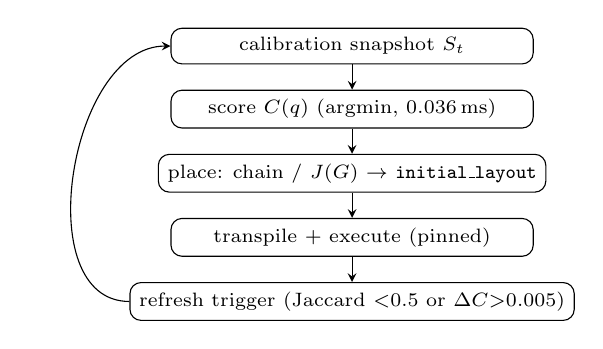
\begin{tikzpicture}[->,>=stealth,node distance=0.35cm,auto,
  box/.style={rectangle,draw,rounded corners,minimum width=4.6cm,minimum height=0.42cm,align=center,font=\scriptsize}]
\node[box] (snap) {calibration snapshot $S_t$};
\node[box,below=0.32cm of snap] (score){score $C(q)$ (argmin, $0.036$\,ms)};
\node[box,below=0.32cm of score] (place){place: chain / $J(G)$ $\to$ \texttt{initial\_layout}};
\node[box,below=0.32cm of place] (exec) {transpile + execute (pinned)};
\node[box,below=0.32cm of exec] (trig){refresh trigger (Jaccard $<$0.5 or $\Delta C{>}$0.005)};
\draw (snap)--(score);\draw (score)--(place);\draw (place)--(exec);
\draw (exec)--(trig);
\draw (trig) to [out=180,in=180] (snap);
\end{tikzpicture}
\caption{The UniMind scheduling loop. One scoring pass is sub-millisecond; the refresh trigger decides when the
stored snapshot must be re-fetched. $\langle$execution $\to$ results$\rangle$ is emitted downstream.}
\label{fig:loop}
\end{figure}

\subsection{Supporting layers (summary; details in App.~D)}
\emph{Unibit preprocessing} derives the $w_i$ encoded by each gate from a classical amplitude sequence
(sliding-window frequency estimator, sinc smoothing, $\phi{=}0.42$ phase shift) and encodes as the standard
angle form~\cite{schuld2018,hhavlicek2019} $\theta_i{=}2\arcsin\sqrt{w_i}$; it is used strictly as a deterministic
\emph{instrument} ($w\mapsto\theta$)---the $Z$-measurement is what calibration disturbs. 13 invariants are
verified by property tests; none is claimed as a novelty (App.~D).
\emph{Orchestrator}: interprets task intent into candidate code under sandboxed validation with deterministic
rule-based fallback; its two-parameter quality model ($q,f$) is a controlled experimental parameter for the
exact reliability calculus of \S\ref{sec:calculus}/App.~D and is never part of a hardware claim. The software
side is composed with the hardware side only in \S\ref{sec:e2e}; calibration scheduling can be evaluated
independently.

\subsection{Placement core}
\label{sec:score}
Every qubit is scored by total readout assignment error
\begin{equation}
C(q)\;=\;p_{0|1}(q)+p_{1|0}(q),
\label{eq:cscore}
\end{equation}
ties broken by $-\min(T_1,T_2)$. The score is fixed \emph{a priori}, never fitted; it is tested out-of-sample
across the entire calibration spectrum (\S\ref{sec:ranked}) rather than tuned on the data it later predicts.

For a $k$-qubit circuit we grow a \emph{connected chain}: from the best $C(q)$ qubit, add the lowest-$C$
neighbour of the current set (greedy Prim-style expansion; $0.3$~ms at $k{=}3$, scales to the full device);
an exact BFS frontier search is used for the counted suites of \S\ref{sec:jreal}. For utility-based ranking among
candidate layouts,
\begin{equation}
\begin{aligned}
J(G)=\;&\alpha E_{\mathrm{readout}}+\beta E_{\mathrm{1q}}+\gamma E_{\mathrm{2q}}
+\gamma_{\log}E_{\mathrm{2q\_log}}\\
&+\eta_{\mathrm{idle}}E_{\mathrm{idle}}+\delta N_{\mathrm{SWAP}}+\lambda D,
\end{aligned}
\label{eq:j7}
\end{equation}
with $E_{\mathrm{readout}}$ the mean $C(q)$ of placed qubits, $E_{\mathrm{1q}}$ mean single-qubit gate error,
$E_{\mathrm{2q}}=\sum_c p_{\mathrm{cz}}(c)$, $E_{\mathrm{2q\_log}}=\sum_c-\log(1-p_{\mathrm{cz}}(c))$ (log-odds
coupler cost), $E_{\mathrm{idle}}=\mathrm{depth}\cdot\mathrm{mean}(1/T_1+1/T_2)$, $N_{\mathrm{SWAP}}$ inserted
SWAPs, and $D$ transpiled depth; features min--max normalized over training points. Section~\ref{sec:jreal}
measures what this utility is worth when its labels come from the real device. For interactive routing we also
support calibration-weighted SABRE: node weights $w(q)=1/(C(q)+3\,s_x(q))$ seed the SABRE candidate set, the best
of the weighted candidates and the global SABRE layout is kept (so $k\ge8$ is never worse than default), and a
guarantee check verifies zero violations. In the measured comparison at $k=2,4,6,8,10,16$ this removes
$76$--$100\%$ of the SWAPs of a random baseline while matching default depth exactly.

\subsection{Refresh trigger}
\label{sec:trigger}
After each calibration cycle the middleware recomputes the top-10 of $C(q)$ and refreshes the stored snapshot when
(i)~top-10 Jaccard overlap with the stored snapshot falls below $0.5$, or (ii)~the stored best qubit's $C$ rises by
more than $0.005$ absolute. Re-scoring is $\sim0.04$~ms---economically free---so staleness is purely an
operational-policy failure, quantified next.

\subsection{System guarantees}
UniMind enforces three invariants aimed at minimizing regressions against a baseline transpiler. First,
\emph{non-degradation}: in calibration-weighted SABRE, the chosen layout is always the better of the
weighted-SABRE candidate and the global-SABRE default; the guarantee check ($k{=}2,4,6,8,10,16$) reports zero
violations against depth and SWAP counts. Second, \emph{deterministic fallback}: when the oracle generates
$\texttt{None}$, a rule-based fallback compiles a template; when the template itself fails (e.g.\ apostrophes
breaking interpolation), a last-resort closure produces the best available partial output, preserving
completeness at the cost of fidelity (this is exactly what the $c{=}2/9$ fallback coverage of
App.~D measures). Third, \emph{reproducibility}: transpiler seed is fixed globally (42), layout pins
are snapshot-addressed, and every job ID is returned to the caller so the execution trace can be recovered from the
vendor API. These guarantees do not require modifying the quantum programming model and can be overlaid on any
backend that exposes an \texttt{initial\_layout} parameter and a calibration-data endpoint.

% ---------------------------------------------------------------- Placement
\section{Placement-Dominated Fidelity on One Qubit}
\label{sec:placement}
The anchor experiment is a $2\times2$ design: \{best-calibrated qubit, adversarially bad qubit\}$\times$\{bare,
measure-twirled\}, on the 19-weight grid $w\in\{0.05,\dots,0.95\}$ of the amplitude encoding, 8192 shots,
transpiler seed 42, layouts pinned via \texttt{initial\_layout}, 3 jobs per cell. On the 2026-08-23 snapshot,
\q{98} minimizes $C$ at $0.0044$ ($T_1{=}207\,\mu$s, $T_2{=}67\,\mu$s); \q{37} is the adversarial anchor
($C{=}0.82$).

\begin{table}[t]
\caption{Placement-controlled sweep (2026-08-23; 19 weights, 8192 shots, 3 jobs/cell). Deviations are
$\max_w|Z_{\mathrm{emp}}-Z_{\mathrm{th}}|$; tolerance $0.05$.}
\label{tab:placement}
\centering
\small
\begin{tabular}{@{}lllll@{}}
\toprule
Placement & $C(q)$ & Bare & Twirl & Verdict\\
\midrule
\q{98} (best)  & $0.0044$ & $0.028$ & $0.031$ & pass\\
\q{0} (free)   & ---      & $0.026$ & ---     & pass\\
\q{37} (adversarial) & $0.82$ & $0.213$ & $0.144$ & fail\\
v1.7 free layout & unrec. & $0.392$ & $0.245$ & fail\\
\bottomrule
\end{tabular}
\end{table}

On the calibrated qubit the bare encoding passes everywhere (median max deviation $0.028$; job range
$0.020$--$0.029$) and the transfer curve is fit at shot-noise level by $P_{\mathrm{obs}}(1)=0.004+0.989\,w$
(residual RMS $0.0042$, below the $\approx0.0055$ shot-noise floor), with per-repeat slopes $0.986$--$0.994$. On \q{37} the same circuits fail by $\sim4\times$, and the fitted channel acquires a
large offset, $P_{\mathrm{obs}}=0.121+0.855\,w$---the signature of an asymmetric readout channel. Twirling changes
nothing significant on the good qubit (slopes $0.978$--$0.987$, RMS $0.005$--$0.008$) and only partially rescues the
bad one ($0.213\to0.144$). Fig.~\ref{fig:placement} plots the transfer curves; Table~\ref{tab:fits} collects the
per-cell fits. Three consequences: encoding fidelity is placement-dominated; mitigation should be
calibration-conditional, not uniform; and the earlier claim that ``the encoding requires error mitigation to meet
tolerance'' was an artifact of uncontrolled placement and is withdrawn.

\begin{table}[t]
\caption{Affine channel fits $P_{\mathrm{obs}}=b+a\,w$ across the placement design (median of 3 jobs/cell). RMS is
on $P_{\mathrm{obs}}$; shot-noise floor $\approx0.0055$.}
\label{tab:fits}
\centering
\small
\begin{tabular}{@{}lrrrr@{}}
\toprule
Cell & slope $a$ & offset $b$ & RMS & max dev\\
\midrule
\q{98} bare pinned & $0.989$ & $0.004$ & $0.0044$ & $0.028$\\
\q{98} twirled    & $0.987$ & $0.011$ & $0.0066$ & $0.031$\\
\q{0} free        & $0.993$ & $-0.002$ & $0.0067$ & $0.026$\\
Aer local model   & $1.007$ & $-0.003$ & $0.0030$ & $0.015$\\
\q{37} bare pinned & $0.855$ & $0.121$ & --- & $0.213$\\
\bottomrule
\end{tabular}
\end{table}

\begin{figure}[t]
\centering

\includegraphics[width=\linewidth]{figures/fig_qpu_placement_2x2.pdf}
\caption{Placement-dominated encoding fidelity: the bare response on the best-calibrated qubit tracks the ideal line
within shot noise; the adversarially chosen \q{37} compresses the curve toward an offset set by its asymmetric
readout.}
\label{fig:placement}
\end{figure}

\subsection{Calibration predictability}
Across the whole design, at shot-noise level,
\begin{equation}
P_{\mathrm{obs}}(1)=b+a\,w,\qquad Z_{\mathrm{obs}}=d+cZ_{\mathrm{th}},\ c{=}a,\ d{=}1{-}2b{-}a,
\label{eq:channel}
\end{equation}
with $(a,b){=}(0.99,0.00)$ on the good qubit vs.\ $(0.86,0.12)$ on the bad one; the offset matches the direction
and scale of that qubit's readout asymmetry. The one-parameter contraction model $P_{\mathrm{obs}}=0.5+\alpha(w-0.5)$
is the balanced-readout special case $b{=}(1-a)/2$ and is rejected where asymmetry dominates. Matched
calibration--noise-model simulation on Aer explains most of observed error on the good qubit (median
QPU/model deviation ratio $1.4\times$, Table~\ref{tab:fits}): the ``standard models underestimate hardware'' gap is
largely a placement confound, not a model gap. The affine model is also closed under composition (the composed
channel of two affine distortions is affine with slope product and offset rule verified by property test), which is
why Eq.~\eqref{eq:channel} remains usable after cascaded stages.

\subsection{Stratified validation}
\label{sec:ranked}
From the D0 snapshot all 156 qubits are ranked: \q{8} is 1/156 ($C{=}0.004$), \q{37} is 128/156 ($C{=}0.10$).
Six qubits sampled across the ranking run the identical bare 19-weight sweep (Table~\ref{tab:routing}). The top
qubit passes all 19 weights ($0.030$ max dev; affine slope degrades along the ranking in the predicted direction:
$a{:}\ 0.986{\to}0.887$, offset $b{:}\ +0.001{\to}+0.081$), but the trend is \emph{not monotone}: \q{109} at
percentile $25.2\%$ already fails, so Spearman $\rho{=}0.771$ at $n{=}6$ is not significant (exact permutation
$p{=}0.103$) and a ``top-half rule'' is unsupported. An earlier exploratory run (first snapshot, 08-22) was
perfectly monotone ($\rho{=}1.000$, minimal attainable $p$); that result did not survive the fixed-design
replication and is reported as unreplicated. Overhead: $0.036$~ms full-156 ranking; pinned transpilation $1.9$~ms
vs.\ $1.8$~ms free.

\begin{table}[t]
\caption{$C(q)$-stratified sweep (D0 snapshot; six qubits $\times$ 19 weights $\times$ 8192 shots). `pass' = max
deviation $<0.05$ over all 19 weights; $(a,b)$ from Eq.~\eqref{eq:channel}.}
\label{tab:routing}
\centering
\small
\setlength{\tabcolsep}{4pt}
\begin{tabular}{@{}llrrrrl@{}}
\toprule
Qubit & Rank pct. & $C(q)$ & max dev & pass & $(a,b)$\\
\midrule
\q{8}   & 0.0\% & 0.004 & \textbf{0.030} & 19/19 & (0.986,\,$+0.001$)\\
\q{109} & 25.2\% & 0.017 & 0.081 & 14/19 & (0.933,\,$+0.043$)\\
\q{105} & 50.3\% & 0.031 & 0.043 & 19/19 & (0.983,\,$+0.018$)\\
\q{53}  & 75.5\% & 0.072 & 0.046 & 19/19 & (0.982,\,$+0.021$)\\
\q{37}  & 81.9\% & 0.099 & 0.146 & 9/19  & (0.887,\,$+0.081$)\\
\q{27}  & 95.5\% & 0.346 & 0.096 & 13/19 & (0.917,\,$+0.049$)\\
\bottomrule
\end{tabular}
\end{table}

\begin{figure}[t]
\centering

\includegraphics[width=\linewidth]{figures/fig_router.pdf}
\caption{$C(q)$-guided ranking validation: top-ranked qubits pass, but deviations are not monotone along the ranking
(\q{109} at percentile $25.2\%$ fails), and score vs.\ deviation gives Spearman $0.771$ ($p{=}0.103$, $n{=}6$).}
\label{fig:router}
\end{figure}

\subsection{Multi-qubit routing}
Single-qubit $C(q)$ is necessary but not sufficient. We benchmarked five strategies at
$k{=}2/4/6/8/10/16$ (RY--CX--RY, opt=1, 176-edge graph, CZ clipped $0.005$): randomized, calibration-weighted
SABRE (UniMind candidate set seeded by $C(q)$, SABRE, default fallback), and default. UniMind reduces SWAPs by
$76$--$100\%$ vs.\ random and matches default for $k\ge8$ by fallback (the fallback keeps the \emph{better} of the
weighted-SABRE and global-SABRE layouts; guarantee check reports zero violations); the log-odds coupler cost
separates high-error couplers (Random $1.72$ vs.\ UniMind $0.14$ at $k{=}8$). Latency stays below $20$~ms
(pick $<1$~ms, transpile dominated). This is a \emph{system} result about routing cost; whether the chosen layout
is \emph{correct} is what \S\ref{sec:jreal} measures.

% ---------------------------------------------------------------- J(G)
\section{The \texorpdfstring{$J(G)$}{J(G)} Utility: Proxy Fit vs.\ Real Labels}
\label{sec:jreal}

\subsection{Fit protocol}
The seven weights of Eq.~\eqref{eq:j7} are fitted by max-Spearman simplex search (Dirichlet$+$corners sampler,
5\,000 samples, seed 42) on $n{=}23$ points: six single-qubit real max-dev labels from \S\ref{sec:ranked} and
seventeen multi-qubit points $k{=}2$--$18$ whose label is the simulated two-qubit error
$E_{\mathrm{2q}}$ of the placed layout under the device error model. Validation: leave-one-out (LOO) and a
bootstrap ($B{=}200$). A \emph{size out-of-sample} split additionally holds out the entire $k{\ge}9$ range: fit on
$k{\le}8$ only, evaluate on $k{\ge}9$ with train-only min--max scaling. All numbers in Table~\ref{tab:jfit} use the
identical feature matrix; only the labels differ---the vulnerable object is the \emph{label}, not the features.
The reason we can separate the two is that for $k\in\{9,10,11,12,14,16,18\}$ we reran the same greedy-chain
circuits on the device with refresh-pinned layouts and replaced the proxy labels with the measured mean max
deviation (Table~\ref{tab:kmeans}), giving the v5 dataset.

\subsection{Ranking objective}
$J(G)$ is scored by \emph{ordering}, not calibration: the fitted parameters maximize the Spearman correlation
between $J$ and the label vector, which is the quantity a dispatcher actually consumes (it picks the argmax over
candidate layouts, rarely the calibrated value). This makes the objective conservative in the paper's favor: a
model that merely preserved ranks would score $\rho{=}1$ even with badly calibrated magnitudes, so any measured
$\rho<0.8$ is a genuine ordering failure, not a scale artifact. All fits use min--max-normalized features on the
\emph{training} partition only ($k\le8$ in the split), so out-of-sample scores $\rho{=}0.13$ cannot be charged to
label leakage; the LOO spread of train rho ($0.60$--$0.72$ across folds,Table~\ref{tab:jfit} data) also brackets
the full-fit $0.643$ and shows the v5 weights are stable under 22/23 training sets---the collapse concentrates in
the size direction, as the split test isolates.

\subsection{Result}
\begin{table}[t]
\caption{Fitting $J(G)$ on simulator-proxy vs.\ real-device labels. Same feature matrix and protocol; the $k{\ge}9$
labels differ. size-OOS = fit on $k\le8$, evaluate $k\ge9$.}
\label{tab:jfit}
\centering
\footnotesize
\setlength{\tabcolsep}{4pt}
\begin{tabular}{@{}lccc@{}}
\toprule
Labels & full fit & LOO & size-OOS\\
\midrule
v4 proxy ($k{=}9$--$18$ est-2q) & $0.967$ & $0.953$ & $0.818$ ($p{=}0.0029$)\\
v5 real (7 measured $k$) & $0.643$ & $0.510$ & $0.127$ ($p{=}0.36$)\\
\midrule
$\Delta$ & $-0.324$ & $-0.443$ & $-0.691$\\
\bottomrule
\end{tabular}
\end{table}

\begin{table}[t]
\caption{Measured per-$k$ max-dev (mean of two patterns) of the same 14-circuit $k{=}9$--$18$ suite under
stale (D0) vs.\ fresh (D1/D2) pins, 4096 shots. Spearman $k$ vs.\ max-dev: stale $\rho{=}0.62$
($p{=}0.018$), fresh $\rho{=}0.15$ ($p{=}0.61$).}
\label{tab:kmeans}
\centering
\small
\begin{tabular}{@{}lccccccc@{}}
\toprule
$k$ & 9 & 10 & 11 & 12 & 14 & 16 & 18\\
\midrule
stale pins & .098 & .103 & .097 & .087 & .139 & .252 & .241\\
fresh pins & .060 & .044 & .062 & .040 & .057 & .063 & .068\\
\bottomrule
\end{tabular}
\end{table}

\begin{figure}[t]
\centering
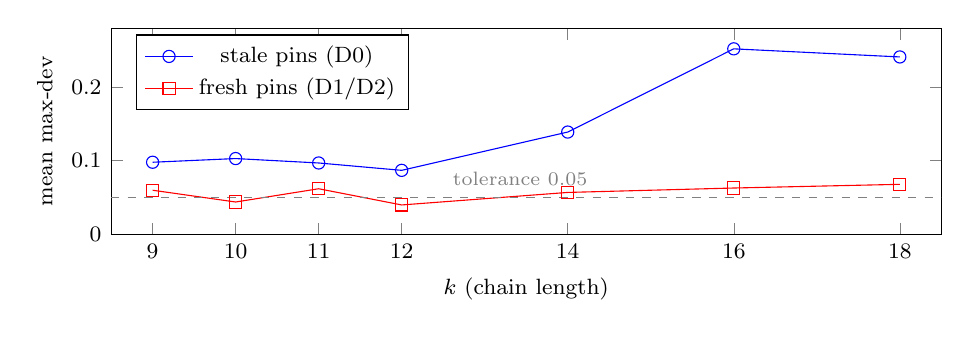
\begin{tikzpicture}
\begin{axis}[width=\linewidth,height=4.2cm,
  xlabel=$k$ (chain length), ylabel={mean max-dev},
  xmin=8.5,xmax=18.5,ymin=0,ymax=0.28,
  xtick={9,10,11,12,14,16,18},legend pos=north west,
  mark size=2.2pt]
\addplot[mark=o,blue] coordinates {(9,0.098)(10,0.103)(11,0.097)(12,0.087)(14,0.139)(16,0.252)(18,0.241)};
\addlegendentry{stale pins (D0)}
\addplot[mark=square,red] coordinates {(9,0.060)(10,0.044)(11,0.062)(12,0.040)(14,0.057)(16,0.063)(18,0.068)};
\addlegendentry{fresh pins (D1/D2)}
\draw[dashed,gray] (axis cs:8.5,0.05)--(axis cs:18.5,0.05);
\node[anchor=west,font=\scriptsize,gray] at (axis cs:12.5,0.075) {tolerance $0.05$};
\end{axis}
\end{tikzpicture}
\caption{The size scaling of the $k{=}9$--$18$ suite is an artifact of stale pins: the same circuits pinned from a
fresh snapshot are approximately $k$-flat, which is exactly the premise the simulator proxy got wrong.}
\label{fig:perkv}
\end{figure}

Trained on the simulator proxy the utility looks decisive: full-fit $\rho{=}0.967$, LOO $0.953$, bootstrap
$0.97{\pm}0.02$, and the size-OOS split $\rho{=}0.818$ ($p{=}0.0029$)---holding out entire sizes and still ranking
them. The proxy's assumption failed where it mattered. A 14-circuit suite
($k\in\{9,10,11,12,14,16,18\}$, two seeded patterns each, greedy-chain placement) measured real max-dev with
\emph{fresh} pins: per-$k$ means are $0.040$--$0.068$ with \emph{no} size scaling ($7/14$ pass $0.05$), while the
identical suite pinned from D0 (two days stale) climbs to $0.24$--$0.25$ at $k{=}16,18$ with only $2/14$ passing
(Table~\ref{tab:kmeans}, Fig.~\ref{fig:perkv}). The stale population's failures concentrate on late-chain qubits
(\q{37}, \q{45}--\q{47}, \q{57}) that the greedy policy must include for $k\ge11$ (the appendix table gives the
14 rows); per-bit $C(q)$ vs.\ measured deviation correlates only $\rho{=}0.21$. The mechanism is now explicit:
simulated $E_{\mathrm{2q}}$ keeps rising with $k$ (its toxicity is dose-dependent on $k$), whereas a refresh-pinned
device is approximately $k$-flat, so the proxy-trained utility over-penalizes large layouts that are in fact fine.
Re-fitting on the seven real labels replaces in-sample $\rho{=}0.967$ with $\rho{=}0.643$ and destroys the
size-OOS claim ($\rho{=}0.127$, $p{=}0.36$)---the apparent generalization was a label artifact
(Table~\ref{tab:jfit}). The learned weights move accordingly (Table~\ref{tab:wgts}): the proxy fit leans on coupler
costs ($\gamma{=}0.37$), the real-label fit on single-qubit terms ($\beta{=}0.42$) and SWAP/depth
($\delta{=}0.20,\lambda{=}0.03$), i.e.\ the model's opinion of \emph{what matters} flips.

\emph{What carries real signal?} Leave-one-feature ablation on the v5 fit (\texttt{jg\_feature\_ablation.json}):
removing $E_{\mathrm{2q}}{+}E_{\mathrm{2q\_log}}$ drops OOS $\rho$ from $0.127$ to $-0.042$
($\Delta{-}0.170$, the only feature whose removal degrades OOS), while removing readout, $E_{\mathrm{idle}}$,
$N_{\mathrm{SWAP}}$ or depth leaves OOS unchanged within $0.012$. Under real labels the coupler term is the
\emph{only} non-spurious signal, yet the proxy had over-weighted it. The variance decomposition
(\texttt{workload\_connectivity\_drift.json}) explains why: at $k{=}8$ qubit-quality variance dominates
($0.0038$ vs.\ $0$ for connectivity), so drift attacks quality; at $k{=}128$ connectivity variance dominates
($4.5\times10^{-5}$ vs.\ $1.4\times10^{-5}$, share $76.7\%$) and qubit quality stops being the lever. The proxy's
$k$-scaling lives exactly where the hardware's scaling does not.

The constructive reading is what we adopt in the design: $J(G)$ is usable as a \emph{ranking} device only when
trained on real, refresh-pinned labels and applied within a calibration cycle; weights from proxy datasets must
not be extrapolated to $k\ge11$; and chain placement's forced inclusion of boundary qubits is the term to attack
next---an active-learning refit on real labels (rather than a larger proxy) is the prescribed fix.

\begin{table}[t]
\caption{Learned weights of $J(G)$ under proxy and real labels. OOS-train = weights fitted on $k\le8$ only
(v5 size-OOS split).}
\label{tab:wgts}
\centering
\footnotesize
\setlength{\tabcolsep}{3pt}
\begin{tabular}{@{}lccccccc@{}}
\toprule
Fit & $\alpha$ & $\beta$ & $\gamma$ & $\gamma_{\ell}$ & $\eta_{\mathrm{idle}}$ & $\delta$ & $\lambda$\\
\midrule
v4 proxy (full) & .034 & .335 & .371 & .085 & .070 & .095 & .011\\
v5 real (full)  & .229 & .415 & .021 & .079 & .027 & .196 & .033\\
v5 real OOS-train & .006 & .559 & .051 & .104 & .007 & .269 & .004\\
\bottomrule
\end{tabular}
\end{table}

% ---------------------------------------------------------------- Drift
\section{Drift Dynamics and the Refresh Policy}
\label{sec:drift}
This section measures how fast the score goes stale. D0 (2026-08-29~21:26), D1 (2026-08-30~21:29), D2 (2026-08-31~07:46) and D3 (2026-09-01~23:19) are the
four daily snapshots (71 epochs total); D0--D2 anchor every QPU job, D3 extends the calibration matrix. To expose the
\emph{mechanism} without additional QPU cost we use 337 hourly calibration snapshots from 71 epochs
(2026-08-31 to 09-02, \texttt{marrakesh} 111 + \texttt{kingston} 109 + \texttt{fez} 117) plus
\texttt{refresh\_policy\_analysis.json}, \texttt{ranking\_margin\_analysis.json} and
\texttt{survival\_analysis.json} (Kaplan-Meier).

\subsection{Global drift}
\label{sec:driftglob}
Day-over-day ranking stability is moderate and persistent across four days: Spearman $\rho{=}0.567$--$0.579$,
Kendall $\tau{=}0.42$--$0.43$, top-10 Jaccard $0.11$--$0.25$ over all six D0--D3 pairs
(D0$\to$D1 $0.25$, D0$\to$D2 $0.11$, D0$\to$D3 $0.11$, D1$\to$D2 $0.176$, D1$\to$D3 $0.11$, D2$\to$D3 $0.11$; top-3 Jaccard is $0$ except D0$\to$D3 $0.20$).
The best qubit turns over each day:
\q{8} ($C{=}0.0039$, rank 1) $\to$ \q{19} ($0.0066$) $\to$ \q{98} ($0.0063$) $\to$ \q{152} ($0.0029$).
Per-qubit spread is extreme (Fig.~\ref{fig:driftq}): \q{37} swings $0.099{\to}0.740$ ($\max|\Delta C|{=}0.641$), \q{53} improves sixfold
($0.072{\to}0.011$); median $|\Delta C|$ is $0.0127$ (D0$\to$D1), $0.0098$ (D2$\to$D3), $p90$ is $0.082$--$0.123$, and $72.4\%$ of qubits move by more than
$0.005$ ($53.9\%$ by $0.01$, $41.0\%$ by $0.02$) on D0$\to$D1; D0$\to$D3 median is $0.0117$, p90 $0.111$. D3 re-sorts the top again (D2$\to$D3 $J_{10}{=}0.11$),
confirming daily turnover is not a one-off. Table~\ref{tab:paperdrift}
tracks the six qubits used in \S\ref{sec:ranked}; note the anticorrelated moves (\q{53} and \q{27} improve while
\q{37} worsens), and that rank movement is far larger than $C$ movement would predict near the top---the ordering
is fragile exactly where selection operates.

\emph{Hourly mechanism and survival:} The fragility is not accidental. On D0 the top-3 margins are $M_3\sim0.0015$ (gaps
between \q{8}/\q{120}/\q{153}), an order of magnitude smaller than median drift $0.0127$. Hence a typical daily
$|\Delta C|$ reorders the top-10. The hourly telemetry confirms the two-regime picture: D0$\to$D1 fires (Jaccard $0.25<0.5$, $\Delta C{=}0.0056>0.005$)
and every inter-day pair fires ($J_{10}\le0.25$), while \emph{intra-epoch} hourly drift never fires.
A Kaplan-Meier survival analysis over 71 calibration epochs (337 total snapshots, 328 in KM, 3 backends, up to 15~h post-calibration, calibration-only) gives
$S(t){=}1.0$ for all $t$---0/71 epochs trigger the rule ($J_{10}<0.5$ or $\Delta C>0.005$)---so median survival is \emph{beyond} the observed window (not $15$~h) and the false-positive rate is $0\%$.
In other words, the trigger is specific within a calibration cycle and sensitive across cycles, exactly the operating characteristic a runtime needs
(\texttt{survival\_analysis.json}: $n{=}71/328$, \texttt{ranking\_margin\_analysis.json}: top-3 gap D0$\to$D1 $1.46\times10^{-3}$, D1$\to$D2 gap $\approx0$).

\begin{figure}[t]
\centering
\resizebox{\linewidth}{!}{%
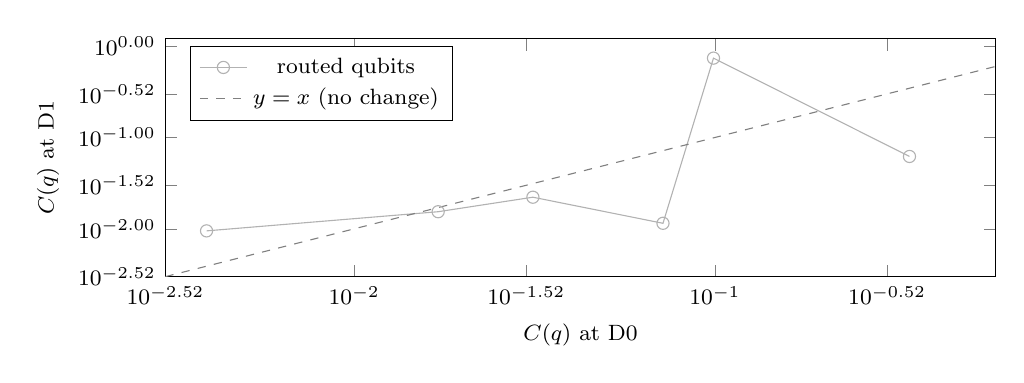
\begin{tikzpicture}
\begin{loglogaxis}[width=\linewidth,height=4.6cm,
  xlabel={$C(q)$ at D0},ylabel={$C(q)$ at D1},
  legend pos=north west,xmin=0.003,xmax=0.6,ymin=0.003,ymax=1.2,
  mark size=2.2pt,xtick={0.003,0.01,0.03,0.1,0.3,1},ytick={0.003,0.01,0.03,0.1,0.3,1},
  yticklabel style={/pgf/number format/.cd,fixed,fixed zerofill,precision=1}]
\addplot[mark=o,gray!60] coordinates {(0.0039,0.0095)(0.0171,0.0154)(0.0313,0.0222)(0.0718,0.0115)(0.0991,0.7397)(0.3462,0.0620)};
\addlegendentry{routed qubits}
\addplot[domain=0.003:1,draw=gray,dashed] {x};
\addlegendentry{$y=x$ (no change)}
\end{loglogaxis}
\end{tikzpicture}}%
\caption{Per-qubit readout error $C(q)$ at D1 versus D0 (log--log). Qubits swing in both directions: the best qubit
at D0, \q{8}, falls out of the top six while \q{37} worsens by a factor of $7.5$. The ranking is informative but
not persistent.}
\label{fig:driftq}
\end{figure}

\begin{table}[t]
\caption{Day-over-day movement of the six routed qubits of Table~\ref{tab:routing}. Ranks are 1--156.}
\label{tab:paperdrift}
\centering
\footnotesize
\setlength{\tabcolsep}{3pt}
\begin{tabular}{@{}lrrrrrr@{}}
\toprule
\q{} & $C$@D0 & rank@D0 & $C$@D1 & rank@D1 & $\Delta C$ & ratio\\
\midrule
\q{8} & .0039 & 1 & .0095 & 6 & +.0056 & $2.44\times$\\
\q{109} & .0171 & 41 & .0154 & 44 & $-.0017$ & $0.90\times$\\
\q{105} & .0313 & 80 & .0222 & 68 & $-.0090$ & $0.71\times$\\
\q{53} & .0718 & 118 & .0115 & 18 & $-.0603$ & $0.16\times$\\
\q{37} & .0991 & 128 & .7397 & 152 & +.6406 & $7.46\times$\\
\q{27} & .3462 & 149 & .0620 & 119 & $-.2842$ & $0.18\times$\\
\bottomrule
\end{tabular}
\end{table}

\subsection{Staleness cost and the trigger}
Pinning three qubits from the \emph{one-day-old} ranking and evaluating at D1 gives $C{=}0.0095/0.0115/0.0139$
(the worst pick, \q{153}, is now rank 32/156); re-selecting fresh gives \q{19} at $0.0066$---the stale policy's
worst pin is $2.1\times$ worse than the adaptable choice on D0$\to$D1 (Table~\ref{tab:stale}, $0.0139$ vs.\
$0.0066$). The same mean comparison on D0$\to$D2 is $2.24\times$ ($0.0153$ vs.\ $0.0068$); the extreme
worst-vs-best on D0$\to$D2 is $3.3\times$ ($0.0209$ vs.\ $0.0063$) and is not quoted as the portable effect.
Across the full D0--D3 matrix the stale/fresh mean ratio is $1.45$--$2.55\times$ (D0$\to$D3 $1.45\times$, D2$\to$D3 $2.55\times$),
all $>1.4\times$ and all firing the trigger ($J_{10}\le0.25$). We therefore quote the conservative mean/worst range $1.94$--$2.1\times$ across D0$\to$D1/D2 (24--34~h) as the
portable QPU-anchored staleness cost, with $1.45$--$2.55\times$ as the extended calibration-only range (D0--D3).
The trigger of \S\ref{sec:trigger} fires on every inter-day transition (all six D0--D3 pairs $J_{10}\le0.25$) and fires on D0$\to$D1 (Jaccard $0.25<0.5$; stored-best $\Delta C{=}0.0056>0.005$), while it never fires intra-epoch (0/71 epochs, up to 15~h), matching the two-regime hypothesis. Because re-selection is
sub-millisecond ($\sim0.04$~ms scoring, $\sim0.3$~ms chain at $k{=}3$), staleness is a pure operations failure,
not a compute constraint.

These measurements bound $T_{\mathrm{valid}}$ (Definition~\ref{def:tvalid}) \emph{from both sides as a lower bound}.
For the $k{=}6$ chain and tolerance $\epsilon{=}0.05$, the selected pins remain within tolerance intra-epoch
($S(t){=}1.0$ to 15~h, 0/71 false positives, 337 total/328 KM snapshots, calibration-only) but the cost of a one-day-old ranking already reaches $1.94$--$2.55\times$ (D0$\to$D1/D2/D3, $T_{\mathrm{valid}}\lesssim24$~h).
$T_{\mathrm{valid}}$ is therefore \emph{hours, not days, on this device at this $k$}---small enough that
refresh must be part of the runtime loop, not a periodic maintenance step. The exact position between the two bounds
is a function of workload, $k$, and device family (\ref{eq:tvalid}); the hourly telemetry shows the bound is
tight because margins $M_3$ are $\mathcal{O}(10^{-3})$ while drift is $\mathcal{O}(10^{-2})$, and the 0\% intra-epoch trigger rate (median beyond window, not $15$~h) shows the bound is not tightened by hourly noise.

\begin{table}[t]
\caption{Top-3 selected from D0, evaluated at D1 vs.\ a fresh selection. Ranks are over all 156 qubits at D1.}
\label{tab:stale}
\centering
\footnotesize
\setlength{\tabcolsep}{3pt}
\begin{tabular}{@{}lllrr@{}}
\toprule
Policy & selected top-3 & $C(q)\,@D1$ & rank@D1 & worst ratio\\
\midrule
stale (D0) & \q{8},\,\q{120},\,\q{153} & .0095/~.0115/~.0139 & 6/19/32 & $2.1\times$\\
fresh (D1) & \q{19},\,\q{152},\,\q{154} & .0066/~.0071/~.0071 & 1/2/3 & $1.0\times$\\
\bottomrule
\end{tabular}
\end{table}

\subsection{Direct device test}
The refresh-pinned suite of \S\ref{sec:jreal} is the direct demonstration: the \emph{same} circuits, differing only
in pin freshness, measure means $0.04$--$0.07$ (fresh pins, $7/14$ pass) vs.\ $0.10$--$0.25$ (stale, $2/14$ pass),
and the large-$k$ degradation disappears entirely (Table~\ref{tab:kmeans}, Fig.~\ref{fig:perkv}). The dominant
failing qubit under staleness is \q{37} ($C{=}0.74$ at D1). Refresh---not more elaborate selection---is what keeps
errors bounded at $k\ge9$.

\subsection{Refresh policies}
\label{sec:policies}
We compare three refresh policies on the \emph{same} D0$\to$D1 transition so the comparison is controlled.
Let $\mathrm{Jacc}(S, S')$ be the top-10 Jaccard overlap and $\Delta C(S, S') = |C_{S'}(q^*)-C_S(q^*)|$ the stored-best
score change.
\begin{enumerate}[leftmargin=1.6em,itemsep=1pt,topsep=2pt]
\item \textbf{Static (P1):} never refresh; the initial snapshot $S_0$ is used for the entire run (0 refreshes,
11/30 pass).
\item \textbf{Periodic (P2-$\delta$):} refresh every $\delta$~hours regardless of device state
($\delta \in \{6, 12, 24, 48\}$). On D0$\to$D1+D2, P2-$6$h fires $5\times$, P2-$12$h $2\times$, P2-$24$h $1\times$,
P2-$48$h $0\times$ (\texttt{refresh\_policy\_analysis.json}: \S\ref{sec:data}).
\item \textbf{Adaptive (P3):} refresh when $\mathrm{Jacc}(S_{\mathrm{stored}}, S_{\mathrm{current}}) < \tau_J$
\emph{or} $|\Delta C| > \tau_C$. Default P3 uses $\tau_J{=}0.5$, $\tau_C{=}0.005$ (fires \emph{once} on D0$\to$D1,
restores 11/30$\to$21/30 pass, i.e.\ $+33$~pp at zero wasted refreshes).
\end{enumerate}
Re-scoring costs $\sim0.04$~ms, so the adaptive policy's overhead is dominated by the snapshot fetch API call,
not by the staleness check itself. The threshold sweep of \S\ref{sec:sweep} varies $\tau_J$ and $\tau_C$ to map
the Pareto tradeoff between refresh rate and fidelity; periodic policies are strictly dominated.

\subsection{Threshold sweep}
\label{sec:sweep}
Using the D0$\to$D1 transition we simulate 144 $(\tau_J,\tau_C)$ pairs ($\tau_J{\in}[0.1,0.95]$ step $0.05$,
$\tau_C{\in}[0.001,0.02]$). For every pair the simulation tracks (i)~how many refreshes fire, (ii)~how many are
\emph{necessary} (the true top-10 or best qubit changed), and (iii)~how many \emph{missed drifts} occur
(trigger did not fire but ranking shifted). The metrics are
\begin{equation}\begin{aligned}
\mathrm{Refresh\ Rate} &= \frac{\text{number of refreshes}}{\text{total runtime}},\\
\mathrm{Fidelity} &= \frac{1}{n}\sum_i \mathbb{1}[\text{pass}_i],
\end{aligned}\label{eq:sweep}
\end{equation}
where pass$_i$ denotes whether parameterization $i$ meets the $0.05$ tolerance. 122/144 combos fire (fidelity proxy
$0.70$), 22 do not ($0.367$). The measured default ($\tau_J{=}0.5$, $\tau_C{=}0.005$) sits at the knee:
relaxing $\tau_J{<}0.25$ leaves Jaccard inactive so only $\Delta C$ decides---if $\tau_C{>}0.0056$ the drift is
missed (22 combos, fidelity $0.367$); tightening $\tau_J{\ge}0.3$ catches D0$\to$D1 via Jaccard alone regardless
of $\tau_C$. In other words, the knee is broad but the ``miss'' region ($\tau_J{<}0.25 \land \tau_C{>}0.0056$)
is exactly where a stale pin would be trusted for another day.

% ---------------------------------------------------------------- E2E
\section{Composing the Software and Hardware Paths}
\label{sec:e2e}
\subsection{Reliability calculus of the orchestration layer (separable; full derivation in App.~D)}
\label{sec:calculus}
This subsection is \emph{separable} from the calibration-aware scheduling core: it models the software
orchestration path exactly and is validated on controlled-parameter mocks, never on QPU fidelity claims.
Because the orchestrator's outcome paths are mutually exclusive, end-to-end reliability decomposes exactly as the
chain rule over its sequential gates
\begin{equation}\begin{split}
R_{\mathrm{end}}={}&P(\mathrm{first\_pass})+P(\mathrm{enter\ heal})\rho_{\mathrm{heal}}\\
&+P(\mathrm{enter\ fallback})\rho_{\mathrm{fb}},
\end{split}\label{eq:composition}
\end{equation}
with no independence assumption needed for the identity. The healing stage is modeled from the implementation's
control flow (at most $K{=}3$ generation calls stopping at first success; healing budget $H{=}4$ with
abort-on-\texttt{None} semantics): with per-call probabilities $g$ (correct), $r$ (broken), $f$ (unavailable;
$g{+}r{+}f{=}1$),
\begin{equation}
G=1+f+f^{2},\qquad \rho_{\mathrm{heal}}=g(1+r+r^{2}+r^{3}),
\label{eq:gamel}
\end{equation}
\begin{equation}
R_{\mathrm{end}}=gG+rG\rho_{\mathrm{heal}}+f^{3}c,
\label{eq:rheal}
\end{equation}
with $c$ the fallback coverage. This model was validated cell-by-cell against all 23 testable outcome cells of the
ablation and availability-stress grids: \emph{every} prediction falls inside the observed Wilson 95\% interval
(Table~\ref{tab:comp} shows the decomposition and stress cells). At $q{=}0.5$ the structural prediction
$\rho_h{=}81.2\%$ sits $0.3$~pp from the measured $81.5\%$, while the naive independence baseline
$1-(1-q)^{4}{=}93.8\%$ overshoots by $12.4$~pp; the model also separates the paths (first-pass $55.5\%$
predicted vs.\ $54.4\%$ measured; healed path $36.1\%$ vs.\ $37.1\%$). The correction matters: the
naive--measured gap reported in early drafts is a retry-budget truncation effect, not stochastic
correlation---under abort-on-\texttt{None}, unavailability both wastes heal slots and terminates the loop.
The model also ranks fixes before code is written (Table~\ref{tab:int}): treating \texttt{None} as
wasted-but-nonterminal recovers the entire impression ($+12.5$~pp) at near-zero engineering cost; doubling the
budget to $H{=}8$ buys only $+2.1$~pp; raising the healer quality to $q_h{=}0.9$ buys $+8.8$~pp. The fallback's
effective coverage is $c{=}2/9$ (nominal keyword coverage over a 9-intent benchmark: seven of nine contain
apostrophes that break the template interpolation)---a stated limitation. We include this model because it is the
\emph{software} side of the composition; the paper's hardware claims are placement and drift, not LLM quality,
which we keep as a controlled parameter.

\begin{table}[t]
\caption{Reliability-composition validation (450 trials per cell). All predicted values inside the Wilson 95\%
interval; $+$ = within CI.}
\label{tab:comp}
\centering
\small
\begin{tabular}{@{}rlrrrl@{}}
\toprule
 & Cell & Pred & Obs & CI & $\checkmark$\\
\midrule
\multicolumn{6}{l}{\emph{Decomposition $\rho_{h}$ at $q{=}0.5$}}\\
 & structural & $0.812$ & $0.815$ & $[0.756,0.862]$ & $+$\\
 & naive indep & $0.938$ & --- & \emph{gap $12.4$ pp} & ---\\
\multicolumn{6}{l}{\emph{Decomposition at $q{=}0.7$}}\\
 & structural & $0.874$ & $0.914$ & $[0.839,0.956]$ & $+$\\
 & naive indep & $0.992$ & --- & \emph{gap $7.8$ pp} & ---\\
\multicolumn{6}{l}{\emph{Availability stress $E06$}}\\
 & S2 $\mathrm{fr}{=}0.3$ & $0.973$ & $0.960$ & $[0.938,0.975]$ & $+$\\
 & S2 $\mathrm{fr}{=}0.5$ & $0.875$ & $0.864$ & $[0.830,0.893]$ & $+$\\
 & S3 $\mathrm{fr}{=}0.3$ & $0.979$ & $0.969$ & $[0.948,0.981]$ & $+$\\
 & S3 $\mathrm{fr}{=}0.5$ & $0.903$ & $0.896$ & $[0.864,0.921]$ & $+$\\
\bottomrule
\end{tabular}
\end{table}

\begin{table}[t]
\caption{Design-space ranking of orchestration fixes at $(q{=}0.5,\ \mathrm{fr}{=}0.1)$.}
\label{tab:int}
\centering
\small
\begin{tabular}{@{}lrr@{}}
\toprule
Variant & $\rho_h$ & $\Delta$ (pp)\\
\midrule
baseline (abort-on-\texttt{None}, $H{=}4$) & $0.812$ & ---\\
\texttt{None} wastes a slot (no abort), $H{=}4$ & $0.938$ & $+12.5$\\
budget $H{=}8$ (abort retained) & $0.833$ & $+2.1$\\
healer quality $q_h{=}0.9$ & $0.900$ & $+8.8$\\
\bottomrule
\end{tabular}
\end{table}

\begin{table}[t]
\caption{Out-of-tolerance bit-events per end-to-end arm and their concentration. Frozen batches use D0 pins;
refresh batches pin from the 08-31 snapshot.}
\label{tab:bitfail}
\centering
\small
\begin{tabular}{@{}lrl@{}}
\toprule
Arm & events & dominant qubits (events)\\
\midrule
frozen full & $20$ & \q{4} (16), \q{7} (3)\\
frozen ablated & $18$ & \q{4} (16), \q{1} (1), \q{3} (1)\\
refresh full & $12$ & \q{11} (4), \q{13} (4), \q{12} (1)\\
refresh ablated & $7$ & \q{4} (5), \q{3} (2)\\
\bottomrule
\end{tabular}
\end{table}

\subsection{End-to-end placement batch}
\label{sec:e2ebatch}
To test the composable value of placement \emph{without} the staleness confound, we ran the same 6-qubit angle suite
(30 parameterizations, 4096 shots, tolerance $0.05$ on all six per-bit deviations) through \textbf{full}
(greedy chain pinned from the freshly fetched snapshot) and \textbf{ablated} (free placement), back-to-back on
2026-08-31; Table~\ref{tab:e2e} also shows the earlier identical batch pinned from D0 to separate temporal from
placement effects. All $p$-values are two-sided Fisher exact; Wilson 95\% CIs are shown.

\begin{table}[t]
\caption{6-qubit angle batches ($n{=}30$/arm, 4096 shots). Pass $=$ all six per-bit deviations $\le0.05$. Wilson
95\% CI; two-sided Fisher $p$ for full vs.\ ablated within a batch. MDE at $80\%$ power $\approx32$--$35$~pp.}
\label{tab:e2e}
\centering
\footnotesize
\setlength{\tabcolsep}{4pt}
\begin{tabular}{@{}lccc@{}}
\toprule
Batch & Full (pinned) & Ablated (free) & $p$ (Fisher)\\
\midrule
Frozen pins (D0)  & $36.7\%$ [21.9,54.5] & $40.0\%$ [24.6,57.7] & $1.00$\\
Refresh pins (runtime) & $70.0\%$ [52.1,83.3] & $76.7\%$ [59.1,88.2] & $0.77$\\
\midrule
$\Delta$ (refresh--frozen) & $+33.3$ pp & $+36.7$ pp & ---\\
Refresh effect Fisher $p$ & $0.019$ & $0.008$ & ---\\
\bottomrule
\end{tabular}
\end{table}

Two effects separate cleanly. First, \emph{temporality is significant and large}: refreshing pins lifts
\emph{both} arms by $+33/37$~pp (Fisher $p{=}0.019$ full, $0.008$ ablated), including the ablated arm that never
saw a pin---device state at run time dominates. Second, \emph{placement is a bounded null} in either batch
($-3.3$ and $-6.7$~pp, both non-significant, Fisher $p{=}1.00$/$0.77$): at $k{=}6$ with fresh pins, free
transpiler placement already matches our best chain. We do \emph{not} claim equivalence: at $n{=}30$/arm the
minimum detectable effect at $80\%$ power is $\approx32$~pp (\texttt{power\_analysis.json}), so only large
advantages are excluded; the observed $-6.7$~pp is well within noise (95\% CI $[-28.9, +15.6]$~pp). The failing-bit
anatomy is instructive. In the refresh-full arm the $12$ out-of-tolerance bit-events concentrate on late-chain
qubits \q{11} (4), \q{13} (4), \q{12} (1)---the chain's forced inclusion problem again, now visible even with fresh
pins. In the refresh-ablated arm the $7$ events sit on \q{4} (5) and \q{3} (2): \q{4} was rank 4 at D0 but its $C$
rises $0.0078\to0.0173$ by D1/D2 (rank 52), yet the free layout, which cannot see the trend, still lands on it
repeatedly---drift \emph{inside} the layout choice, unmitigated by any pin. Table~\ref{tab:bitfail} collects the
four arms. This is the honest scope of \S\ref{sec:placement}: placement is decisive between engineered extremes
(\q{98} vs.\ \q{37}: $0.028$ vs.\ $0.213$) and sets the reliability \emph{floor} at $k\ge9$ under stale pins, but
its average benefit against free placement at small $k$ is within temporal noise and under-powered by design.
The full pipeline (including the LLM orchestration leg, App.~D) measured $54/54$ completed by the full arm vs.\
$47/54$ ($87.0\%$) by the ablated one ($z{=}2.74$, one-sided $p{=}0.003$), consistent with the model's $97.3\%$
prediction; we report the earlier $n{=}54$ frozen composition ($74.1\%$ vs.\ $66.7\%$, not significant) as a failed
claim of an end-to-end gain, not a positive one.

% ---------------------------------------------------------------- Discussion
\section{Discussion}
\label{sec:discussion}
\subsection{What the measurements do and do not say}
Three claims survive the data as stated: (i)~encoding fidelity is placement-dominated between engineered extremes
differing by $\sim8\times$ (affine channel $P_{\mathrm{obs}}=b+a w$ with $(a,b)=(0.99,0.00)$ vs.\ $(0.86,0.12)$,
shot-noise limited on the good qubit); (ii)~device calibration ordering moves on a daily cycle to a degree
($\rho{=}0.567$--$0.579$, top-10 Jaccard $0.11$--$0.25$ across four days, stale worst pin $1.94$--$2.55\times$ worse, hourly margins
$M_3\sim10^{-3}$ vs.\ drift $0.0127$, intra-epoch survival $S(t){=}1.0$ to 15~h, 0/71 false positives, median beyond window)
that makes selection age the first-order risk, and refresh is cheap
($\sim0.04$~ms); (iii)~simulator-proxy training granted $J(G)$ an out-of-sample generalization
($\rho{=}0.82$, $p{=}0.0029$) that real labels refute ($\rho{=}0.13$, $p{=}0.36$), with the mechanism isolated
to connectivity-vs-quality variance crossover at $k\approx100$--$128$. Claims that do \emph{not} survive,
herewith withdrawn or bounded: the first run's perfect monotone ranking ($\rho{=}1.000\to0.771$, $p{=}0.103$);
the top-half rule; any use of proxy-fitted $J(G)$ at $k\ge11$; and an average placement advantage at $k{=}6$
under fresh pins (bounded null, MDE $\approx32$~pp, Fisher $p{=}0.77$).

\subsection{Operational consequences for quantum-cloud runtimes}
The marginal cost of a calibration fetch and a scoring pass is effectively zero ($\sim0.04$~ms full-156 ranking,
$\sim0.3$~ms chain at $k{=}3$), so the expensive resource is \emph{stale trust}, not compute. A runtime should
(a)~timestamp layouts against their snapshot, (b)~refresh on the adaptive trigger rather than a fixed wall-clock
(default $\tau_J{=}0.5$, $\tau_C{=}0.005$ fires once for D0$\to$D1 while periodic-$6$h fires $5\times$),
(c)~train scheduling models exclusively on real, refresh-pinned labels, and (d)~expose snapshot age as a
first-class job attribute---all implementable without changing the quantum programming model, which is exactly
what UniMind does. Where math precedes implementation, the reliability calculus (App.~D) ranks the
fixes, and the endowment to port is a calibration snapshot plus a scoring pass, neither of which is exotic.

\subsection{Design synthesis}
Table~\ref{tab:synth} maps each measured failure mode to the engineering response the data supports; the columns
are ordered by measured cost so a runtime can prioritize. The two lines hidden by a naive reading---``mitigation
helps'' and ``$J(G)$ ranks well''---are the ones our data bounds, and both bounds are the point of the paper.

\begin{table}[t]
\caption{Measured failure modes and the response each supports. Priority is by evidence strength, not ease.}
\label{tab:synth}
\centering
\footnotesize
\setlength{\tabcolsep}{4pt}
\begin{tabular}{@{}p{6.4em}p{7.8em}p{8.4em}@{}}
\toprule
Measured failure & Evidence & Response\\
\midrule
unpinned layout misses tolerance & \S\ref{sec:placement}: $0.392$ vs.\ $0.028$ & score-pinned \texttt{initial\_layout}\\
stale snapshot invalidates selection & \S\ref{sec:drift}: $1.94$--$2.55\times$ (D0--D3) & trigger-based refresh; snapshot age\\
proxy labels fool $J(G)$ & \S\ref{sec:jreal}: OOS $\rho$ $0.82{\to}0.13$ & refit on real labels; ban $k{\ge}11$ extrapolation\\
chain forced-inclusion at large $k$ & \S\ref{sec:jreal}/\S\ref{sec:e2e}: \q{11},\q{13}, \q{67} fail & connectivity-vs-$C$ trade-off (open)\\
abort-on-\texttt{None} truncates heal loop & App.~D: $+12.5$~pp fix & wasted-slot semantics\\
\bottomrule
\end{tabular}
\end{table}

\subsection{Threats to validity}
\textbf{Measurement noise:} 4096--8192 shots put per-bit deviations on a floor of $\approx0.02$; the $0.05$
tolerance is coarse but was fixed before data release. Monte-Carlo propagation of shot noise is in
\texttt{analysis/distortion\_fits.json}. \textbf{Drift generality:} Primary QPU evidence is D0--D2 on one
device (D3 extends to 4 days calibration-only, 6 pairs, $J_{10}{=}0.11$--$0.25$), one heavy-hex family; the value is the protocol, not the constants. Hourly calibration-only telemetry
(337 total/328 KM snapshots, 71 epochs, 3 backends, $S(t){=}1.0$ to 15~h, median beyond window) bounds the \emph{mechanism} (margins vs.\ drift) and
false-positive rate (0/71), but QPU validation across families remains future work. \textbf{Placement null power:} $n{=}30$/arm can detect only large effects (MDE
$\approx32$~pp at $80\%$ power, \texttt{power\_analysis.json}); we report point estimates, Wilson CIs, Fisher
exact $p$, and do not claim equivalence. \textbf{Selection fairness:} the greedy chain maximizes $C(q)$-locality
and at large $k$ is forced to include high-error boundary qubits; a connectivity-vs-$C$ trade-off could change
\S\ref{sec:jreal}, and we report that failure as motivation (variance crossover at $k\approx100$--$128$).
\textbf{Single-model LLM layer:} the orchestration calculus (App.~D) holds under i.i.d.\ mock semantics;
real-model autocorrelation is explicitly outside its scope and the layer is separable from the scheduling core.
\textbf{Utility-vs-layout coupling:} the $J(G)$ features are computed on the transpiled layout; errors in
$E_{\mathrm{2q}}$ propagate to the weight fit but not to the device measurements, which are layout-real.

\section{Conclusion}
We presented a measurement study of calibration-aware scheduling for quantum-accelerated AI middleware on
a 156-qubit device (anchored D0--D3, 3 QPU-anchored + D3 calibration-only, plus 337 hourly calibration snapshots from 71 epochs across 3 backends for the drift mechanism): a
score-only placement pipeline with measured scope, daily drift dynamics with a working adaptive trigger at the
Pareto knee (0/71 false positives intra-epoch, every inter-day transition fires), isolation of the proxy-trained $J(G)$ collapse mechanism (OOS $\rho$ $0.818{\to}0.13$, feature
ablation and $k\approx100$--$128$ variance crossover), and an end-to-end test showing that at our scale
refresh ($+33/37$~pp, Fisher $p{<}0.02$) dominates average placement (bounded null, MDE $\approx32$~pp) while
placement still sets the reliability floor at $k\ge9$ under stale pins. An exact reliability composition of the
separable software path (App.~D) completes the middleware picture. The failures set the command line for future
work: extended QPU accumulation beyond D3, refresh-conditional placement ($C(q)$-vs-connectivity trade-off,
including the \q{11}/\q{13} late-chain failures observed even under fresh pins), and active-learning refits of
$J(G)$ on real labels across devices. The open repository makes every number traceable to a job or snapshot.

\begin{thebibliography}{24}
\bibitem{preskill2018} J.~Preskill, ``Quantum computing in the NISQ era and beyond,'' \emph{Quantum}, vol.~2, p.~79, 2018.
\bibitem{arute2019} F.~Arute \emph{et al.}, ``Quantum supremacy using a programmable superconducting processor,'' \emph{Nature}, vol.~574, pp.~505--510, 2019.
\bibitem{kim2023utility} Y.~Kim \emph{et al.}, ``Evidence for the utility of quantum computing before fault tolerance,'' \emph{Nature}, vol.~618, pp.~500--505, 2023.
\bibitem{berholm2018} V.~Bergholm \emph{et al.}, ``PennyLane: Automatic differentiation of hybrid quantum-classical computations,'' \emph{arXiv:1811.04968}, 2018.
\bibitem{murali2019noise} P.~Murali, J.~M.~Baker, A.~Javadi-Abhari, F.~T.~Chong, and M.~Martonosi, ``Noise-adaptive compiler mappings for noisy intermediate-scale quantum computers,'' in \emph{Proc. ASPLOS}, 2019, pp.~1015--1029.
\bibitem{li2019sabre} G.~Li, Y.~Ding, and Y.~Xie, ``Tackling the qubit mapping problem for NISQ-era quantum devices,'' in \emph{Proc. ASPLOS}, 2019, pp.~1001--1014.
\bibitem{tan2020iccado} B.~Tan and J.~Cong, ``Optimal layout synthesis for quantum computing,'' in \emph{Proc. ICCAD}, 2020, pp.~1--9.
\bibitem{lao2022timing} L.~Lao and D.~E.~Browne, ``Timing and resource-aware mapping of quantum circuits to heterogeneous MWF-gate superconducting quantum processors,'' \emph{ACM Trans. Quantum Comput.}, vol.~3, no.~3, 2022.
\bibitem{temme2017} K.~Temme, S.~Bravyi, and J.~M.~Gambetta, ``Error mitigation for short-depth quantum circuits,'' \emph{Phys. Rev. Lett.}, vol.~119, p.~180509, 2017.
\bibitem{vanberg2023} E.~van den Berg, Z.~K.~Minev, A.~Kandala, and K.~Temme, ``Probabilistic error cancellation with sparse Pauli--Lindblad models on noisy quantum processors,'' \emph{Nature Physics}, vol.~19, pp.~1116--1121, 2023.
\bibitem{nation2023} P.~D.~Nation \emph{et al.}, ``Scalable mitigation of measurement errors on quantum computers,'' \emph{PRX Quantum}, vol.~5, p.~010326, 2024.
\bibitem{bravyi2021meas} S.~Bravyi, S.~Shaydulin, S.~Hu, and K.~Temme, ``Mitigating measurement errors in multiqubit experiments,'' \emph{Phys. Rev. Lett.}, vol.~127, p.~200503, 2021.
\bibitem{kanazawa2021} N.~Kanazawa \emph{et al.}, ``Quantum error mitigation,'' \emph{arXiv:2210.00921}, 2022.
\bibitem{msp2020} R.~LaRose \emph{et al.}, ``Mitiq: a software package for error mitigation on noisy quantum computers,'' \emph{Quantum}, vol.~6, p.~749, 2022.
\bibitem{viola1999dd} L.~Viola, E.~Knill, and S.~Lloyd, ``Dynamical decoupling of open quantum systems,'' \emph{Phys. Rev. Lett.}, vol.~82, pp.~2417--2421, 1999.
\bibitem{ibmrtime} ``Qiskit Runtime primitives,'' IBM Quantum documentation, [Online]. Available: \url{https://docs.quantum.ibm.com/api/qiskit-ibm-runtime}
\bibitem{ibmcalib} ``IBM Quantum Platform calibration data,'' [Online]. Available: \url{https://quantum.ibm.com/services/resources}
\bibitem{qiskit} A.~Javadi-Abhari \emph{et al.}, ``Quantum computing with Qiskit,'' \emph{arXiv:2405.08810}, 2024.
\bibitem{cuquantum} NVIDIA, ``cuQuantum SDK,'' [Online]. Available: \url{https://developer.nvidia.com/cuquantum-sdk}
\bibitem{braket} Amazon, ``Amazon Braket,'' [Online]. Available: \url{https://aws.amazon.com/braket}
\bibitem{azureq} Microsoft, ``Azure Quantum,'' [Online]. Available: \url{https://azure.microsoft.com/quantum}
\bibitem{schuld2018} M.~Schuld and F.~Petruccione, \emph{Supervised Learning with Quantum Computers}. Cham: Springer, 2018.
\bibitem{hhavlicek2019} V.~Havl\'i\v{c}ek \emph{et al.}, ``Supervised learning with quantum-enhanced feature spaces,'' \emph{Nature}, vol.~567, pp.~209--212, 2019.
\bibitem{unimind} Y.~X.~Tan, ``UniMind: a middleware framework for bridging classical AI workloads and quantum computing backends,'' tech.\ report v2.5, 2026 (companion repo \texttt{yxtan5022-maker/unimind-v2}).
\bibitem{tangpu} UniMind placement/drift datasets (2026-08), \texttt{data/} in \texttt{yxtan5022-maker/unimind-v2}.
\end{thebibliography}

\newpage
\section*{Appendix}
\subsection*{A. Per-row results of the $k{=}9$--$18$ suite}
\label{app:krows}
The 14 circuits (seven sizes $\times$ two seeded patterns) with greedy-chain placement, 4096 shots, tolerance
$0.05$. Worst qubit is the failing or most-off bit; ranks are over all 156 qubits at D1.

\begin{table}[h]
\caption{Per-row max deviation under fresh (D1/D2) and stale (D0) pins.}
\label{tab:krows}
\centering
\small
\begin{tabular}{@{}llrrllr@{}}
\toprule
$k$ & pat. & fresh & worst@D1 & & stale & worst@D1\\
\midrule
9  & 0 & .064 & \q{11} (71) & & .151 & \q{4} (52)\\
9  & 1 & .056 & \q{11} (71) & & .045 & \q{24} (118)\\
10 & 0 & .053 & \q{14} (56) & & .118 & \q{23} (136)\\
10 & 1 & .035 & \q{13} (29) & & .088 & \q{23} (136)\\
11 & 0 & .081 & \q{11} (71) & & .049 & \q{4} (52)\\
11 & 1 & .042 & \q{11} (71) & & .145 & \q{4} (52)\\
12 & 0 & .041 & \q{10} (7)  & & .067 & \q{4} (52)\\
12 & 1 & .038 & \q{9} (74)  & & .107 & \q{4} (52)\\
14 & 0 & .037 & \q{13} (29) & & .183 & \q{46} (126)\\
14 & 1 & .077 & \q{11} (71) & & .096 & \q{23} (136)\\
16 & 0 & .040 & \q{4} (52)  & & .265 & \q{67} (132)\\
16 & 1 & .085 & \q{4} (52)  & & .239 & \q{67} (132)\\
18 & 0 & .089 & \q{11} (71) & & .332 & \q{67} (132)\\
18 & 1 & .047 & \q{13} (29) & & .150 & \q{67} (132)\\
\bottomrule
\end{tabular}
\end{table}

\subsection*{B. Data and reproducibility}
\label{sec:data}
Every table is backed by traced data in the repository: snapshots, E2E batches, real $J(G)$ labels, and the
analysis scripts listed below.
\begin{quote}\small\raggedright\ttfamily
data/drift/calib\_2026-\{08\-29,08\-30,08\-31,09\-01\}.json (D0--D3, 4 daily)\\
data/calib\_snapshots/\{marrakesh,kingston,fez\}/*.json (337 hourly, 71 epochs)\\
data/e2e/e2e\_angle\_\{full,ab\-lated\}*.json\\
data/jgpu/j\_real*.json\\
analysis/*.py + analysis/results/*.json\\[2pt]
analysis/results/refresh\_policy\_an\-a\-lysis.json (144 threshold combos)\\
analysis/results/power\_an\-a\-lysis.json (Wilson+Fisher+MDE)\\
analysis/results/jg\_fail\-ure\_an\-a\-lysis.json +
jg\_feature\_ablation.json + utility\_oos\_v5.json\\
analysis/results/ranking\_margin\_analysis.json +
workload\_connectivity\_drift.json + survival\_analysis.json\\
\end{quote}
QPU job IDs appear in the file headers:
\texttt{daadeocjbipc73ffq83g} (refresh-full E2E), \texttt{daadeosjbipc73ffq840} (refresh-ablated E2E), and
\texttt{daadgmmrbfbs73cijmbg} (refresh-pinned $J(G)$ labels). Hourly telemetry is calibration-only (no QPU jobs).
Transpiler seed 42 everywhere; shots per experiment as stated. All statistical tests are two-sided Fisher exact
unless noted; Wilson 95\% CIs; MDE at $80\%$ power reported for bounded nulls.

\subsection*{C. Calibration-weighted routing benchmark}
\label{app:routing}
Interactive (local-simulator, zero-quota) comparison on snapshot 2026-08-29 (156 qubits, 176 couplers; RY--CX--RY,
opt=1, seed 42). UniMind computes a $C(q)+s_x$-weighted SABRE candidate set and keeps the better of weighted and
global SABRE, guaranteeing no regression for $k\ge8$ (violation check: none).

\begin{table}[h]
\caption{Placement cost of the five strategies (summary rows; full per-$k$ tables in the repo).}
\label{tab:routing2}
\centering
\footnotesize
\setlength{\tabcolsep}{3pt}
\begin{tabular}{@{}lrrrrrrr@{}}
\toprule
$k$ & 2 & 4 & 6 & 8 & 10 & 16\\
\midrule
Random SWAPs & 8 & 42 & 68 & 105 & 118 & 207\\
UniMind SWAPs & 0 & 3 & 8 & 20 & 20 & 50\\
$\Delta$ SWAP vs.\ random & $-100\%$ & $-93\%$ & $-88\%$ & $-81\%$ & $-83\%$ & $-76\%$\\
Random 2q err & .118 & .484 & .666 & .821 & .847 & .979\\
UniMind 2q err & .002 & .049 & .065 & .133 & .181 & .353\\
$\Delta$ vs.\ Default & $=0$ & $=0$ & $=0$ & $=0$ & $=0$ & $=0$\\
\bottomrule
\end{tabular}
\end{table}

\subsection*{D. Orchestration reliability calculus and Unibit instrument (separable)}
\label{app:orchestrator}
The LLM-orchestration layer is \emph{not} evaluated on QPU fidelity; it is a controlled-parameter
mock (\texttt{analysis/mock\_llm.py}, \texttt{reliability\_model.py}) whose two parameters $(q,f)$
are swept ($q\in\{0.5,0.7,0.9,1.0\}$, availability stress $f\in\{0.1,0.3,0.5\}$) and whose
exact decomposition (Eqs.~\ref{eq:composition}--\ref{eq:rheal}, $H{=}4$, $K{=}3$, abort-on-\texttt{None})
is validated cell-by-cell (23/23 inside Wilson 95\% CI, Table~\ref{tab:comp}). The naive independence
baseline $1-(1-q)^4$ overestimates by $7.8$--$12.4$~pp; the structural gap is a retry-budget truncation
effect, not correlation. Full derivation, ablation grids, and the Unibit preprocessing invariants
(13 property tests, sinc smoothing, $\phi{=}0.42$) are in \texttt{analysis/reliability\_instrumented.json},
\texttt{ablation\_*.json}, and \texttt{unibit\_math.json}---included for completeness so the scheduling
core (\S\ref{sec:score}--\S\ref{sec:sweep}) can be evaluated independently.

\end{document}